\documentclass{article}
\usepackage{graphicx}
\usepackage[margin=1.5cm]{geometry}
\usepackage{csquotes}

\begin{document}
\twocolumn

\title{Monday Warm-Up: Chapters 18-22 of \textit{Last Place on Earth}}
\author{Prof. Jordan C. Hanson}

\maketitle

\section{Chapter 18 - Volte-Face}

\begin{enumerate}
\item Cpt. Amundsen chose to land and establish winter quarters not on firm land, but on the \textit{Ross Ice Shelf itself.}  (a) Why did he do this?  (b) The landing point of Amundsen and his companions was about 1.0 degree of latitude closer to the pole than Robert Falcon Scott.  What distance is this in kilometers? \\ \vspace{3cm}
\item What skill did Roald Amundsen and his men have to learn in order to study the work of Ernest Shackleton in his attempt on the South Pole on the \textit{Nimrod} expedition?  What conclusions did they draw regarding margins of error? \\ \vspace{3cm}
\end{enumerate}

\section{Chapter 19 - On the Terra Nova}

\begin{enumerate}
\item Part of Robert Falcon Scott's plan for tackling the surface travel from McMurdo sound to the South Pole was the \textit{motor sledge.}  Describe the scene when they first tested the complete prototype near Christiania.  What problem occurred, and how did they remedy the situation?  What was to be learned from this situation? \\ \vspace{3cm}
\item Although Scott tried to meet with Amundsen to learn new things about the Antarctic, Amundsen managed to avoid Scott while Scott was in Christiania.  Why did Amundsen do this? \\ \vspace{2cm}
\end{enumerate}

\section{Chapter 20 - The Secret Disclosed}
\begin{enumerate}
\item Describe the scene when Amundsen boarded the \textit{Fram} and left for Antarctica.  From where did they leave, and what strange equipment did they stow aboard? \\ \vspace{2cm}
\item Describe the scene as Amundsen revealed his secret plan to reach the South Pole to his shipmates.  How did they respond?  What does this tell us about his leadership style?  \\ \vspace{2cm}
\item There is an interesting detail about \textit{wireless} (they mean radio communications).  What about the race to the pole between Scott and Amundsen, and the press, would have changed if Scott had set up wireless communications to New Zealand? \\ \vspace{2cm}
\end{enumerate}

\section{Chapter 21 - Scott Sails On}

\begin{enumerate}
\item Robert Falcon Scott selected which draught animal to help pull the sledges?  From where did they acquire them?  Why was this especially difficult, logistically? \\ \vspace{2cm}
\item Do you recall the story of the \textit{the broken pump}?  The Terra Nova is sailing through that dangerous part of the ocean between New Zealand and Antarctica.  The ship is equipped with a broken water pump.  What happened next?  How did the ship and crew survive? \\ \vspace{2cm}
\end{enumerate}

\section{Chapter 22 - The Base at Framheim}

\begin{enumerate}
\item
\begin{figure}[hb]
\centering
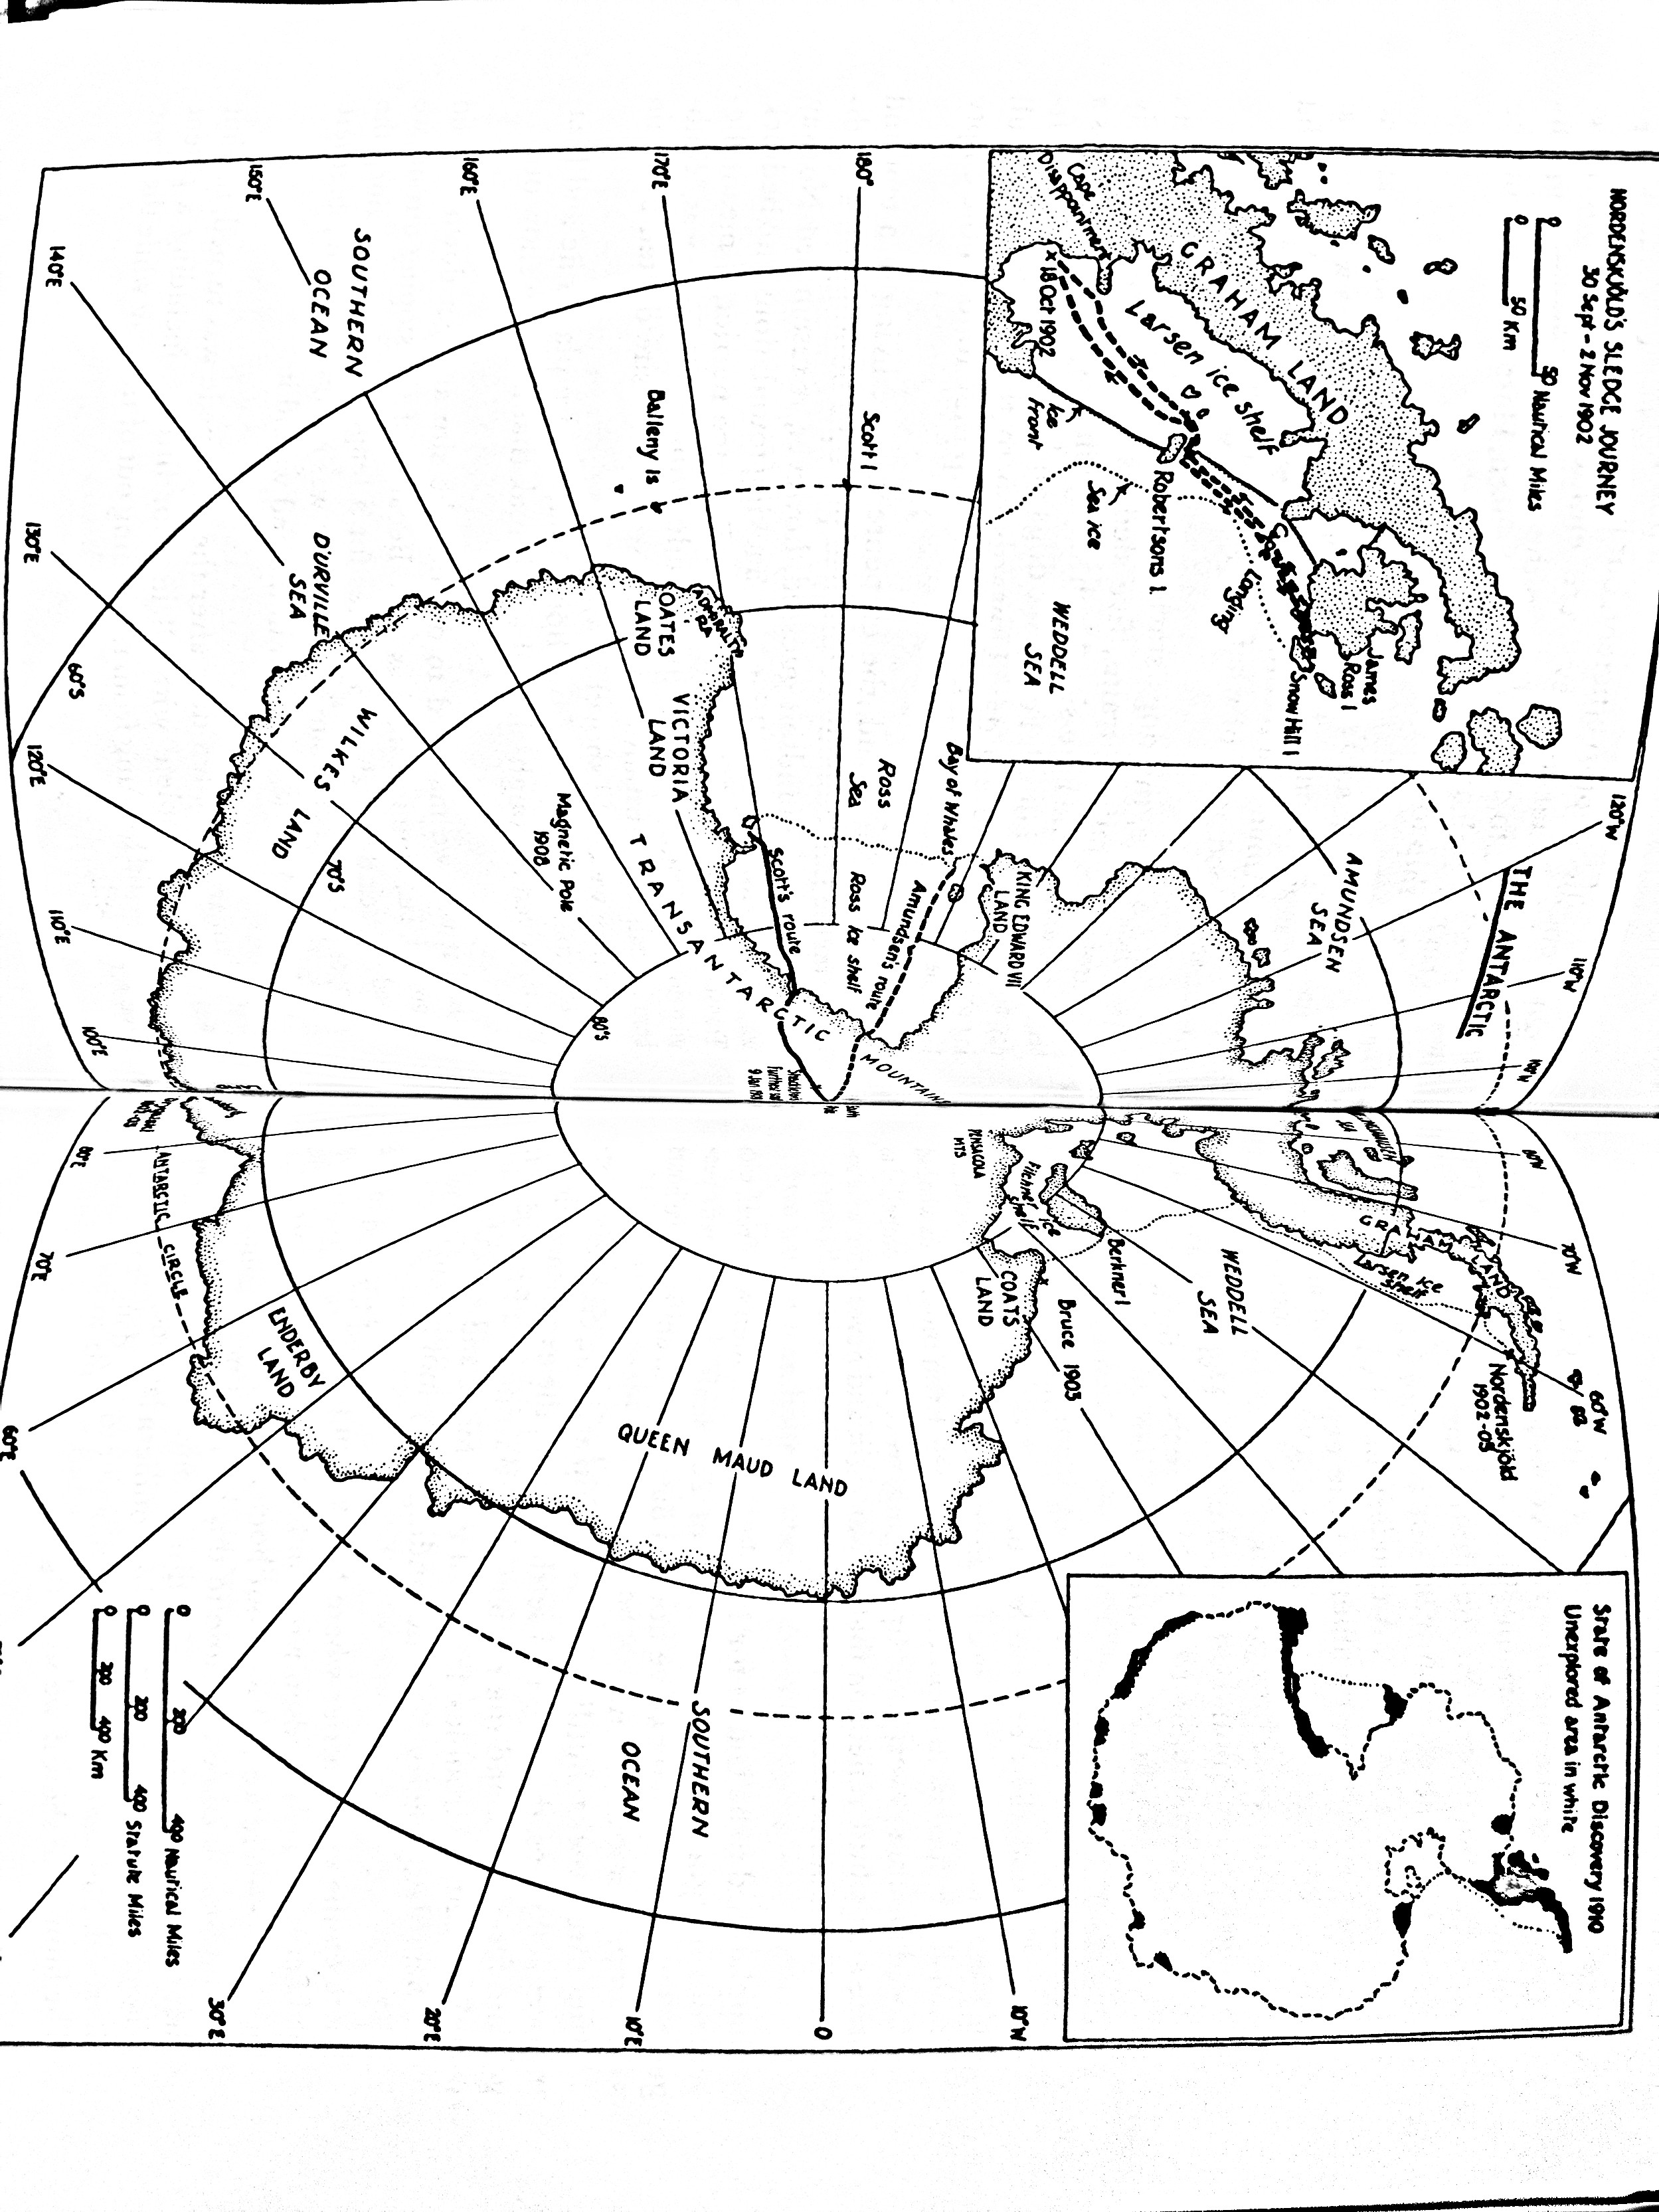
\includegraphics[width=0.3\textwidth,angle=90,trim=1cm 1cm 1cm 1cm,clip=true]{Map.jpg}
\caption{\label{fig:Map} A map from Ch. 21 showing the pathways of the two explorers to the South Pole.}
\end{figure}
In Fig. \ref{fig:Map}, we see the two landing points of the two South Pole seeking groups.  Do you see how they are choosing the closest landing points possible to South Pole?  Answer the following questions about the map.  (a) Where is Scott landing?  (b) Where is Amundsen landing?  (c) Which proposed pathway is longer? \\ \vspace{2cm}
\end{enumerate}

\end{document}
